\documentclass{article}
\usepackage[utf8]{inputenc}
\usepackage[margin = 0.8in]{geometry}
\usepackage{graphicx}
\usepackage{amsmath, amssymb}
\usepackage{subcaption}
\usepackage{multirow}
\usepackage{mathtools}
\usepackage{float}
\usepackage{pythonhighlight}


\title{RBE595 - Homework 1}
\author{Keith Chester}
\date{Due date: January 15, 2024}

\begin{document}
\maketitle

In this assignment we are provided with a proposed system of a drone tracked by a series of motion capture cameras. We are asked to formulate the system dynamics and Kalman Filter for this system, and then provided a set of measurements from the system for testing out implementation.

CSV files are provided that provide measurements - some in velocity, others direct position.

The system dynamics are given as:

\begin{equation}
    \textbf{x} = \begin{bmatrix}
        p \\ \dot{p}
    \end{bmatrix} =
    \begin{bmatrix}
        x       \\ y \\ z \\
        \dot{x} \\ \dot{y} \\ \dot{z}
    \end{bmatrix}
\end{equation}

...and inputs in the form of

\begin{equation}
    \textbf{u} = m \textbf{$\ddot{p}$}
\end{equation}

...wherein $m$ is our drone mass, at $27$ grams. We are instructed to assume that all noise is additive Gaussian noise with 0 mean and a diagonal covariance matrix since the form of $\Sigma=\sigma^2 I$. The noise has $\sigma=0.05$ m for low noise, $\sigma=0.20$ m for high noise, and $\sigma=0.05$ m/s for velocity noise.

\section*{Task 1}

In this task we are asked to determine the matricies used in the process and measurement models, ignoring the noise matricies.

First we start with our state and known equations for our state and motion:

\begin{equation}
    \textbf{x} = \begin{bmatrix}
        p \\ \dot{p}
    \end{bmatrix} =
    \begin{bmatrix}
        x       \\ y \\ z \\
        \dot{x} \\ \dot{y} \\ \dot{z}
    \end{bmatrix}
\end{equation}

...and we know the state model for motion is:

\begin{equation}
    \begin{split}
        x = x + \frac{dx}{dt} + \frac{dx}{dt^2} \\
        y = y + \frac{dy}{dt} + \frac{dy}{dt^2} \\
        z = z + \frac{dz}{dt} + \frac{dz}{dt^2} \\
        \dot{x} = \dot{x} + \frac{d\dot{x}}{dt} \\
        \dot{y} = \dot{y} + \frac{d\dot{y}}{dt} \\
        \dot{z} = \dot{z} + \frac{d\dot{z}}{dt} \\
    \end{split}
\end{equation}

...which we can also express in discrete terms:

\begin{equation}
    \begin{split}
        x = x + \dot{x} \Delta t + \frac{1}{2} \ddot{x} \Delta t^2 \\
        y = y + \dot{y} \Delta t + \frac{1}{2} \ddot{y} \Delta t^2 \\
        z = z + \dot{z} \Delta t + \frac{1}{2} \ddot{z} \Delta t^2 \\
        \dot{x} = \dot{x} + \ddot{x} \Delta t \\
        \dot{y} = \dot{y} + \ddot{y} \Delta t \\
        \dot{z} = \dot{z} + \ddot{z} \Delta t \\
    \end{split}
\end{equation}

We wish to find the matricies in the following equation:

\begin{equation}
    \textbf{$\dot{x}$} = \textbf{F} \textbf{x} + \textbf{G} \textbf{u} + E \eta
\end{equation}


Since we are ignoring process noise, we can drop $E \eta$ from the equation. Solving for the $\textbf{F}$ matrix:

\begin{equation}
    \textbf{F} = \begin{bmatrix}
        1 & 0 & 0 & \Delta t & 0        & 0        \\
        0 & 1 & 0 & 0        & \Delta t & 0        \\
        0 & 0 & 1 & 0        & 0        & \Delta t \\
        0 & 0 & 0 & 1        & 0        & 0        \\
        0 & 0 & 0 & 0        & 1        & 0        \\
        0 & 0 & 0 & 0        & 0        & 1        \\
    \end{bmatrix}
\end{equation}

...this is derived from an understanding of our state equations above.

For our \textbf{G} matrix, we first look at our $\textbf{u}$ state equation:

\begin{equation}
    \textbf{u} = m \textbf{$\ddot{p}$}
\end{equation}

...thus $\textbf{$\ddot{p}$}$ can be isolated:

\begin{equation}
    \textbf{$\ddot{p}$} = \frac{\textbf{u}}{m}
\end{equation}

...so our G equation would be:

\begin{equation}
    \textbf{G} = \begin{bmatrix}
        \frac{\Delta t^2}{2m} & 0                     & 0                     \\
        0                     & \frac{\Delta t^2}{2m} & 0                     \\
        0                     & 0                     & \frac{\Delta t^2}{2m} \\
        \frac{\Delta t}{m}    & 0                     & 0                     \\
        0                     & \frac{\Delta t}{m}    & 0                     \\
        0                     & 0                     & \frac{\Delta t}{m}    \\
    \end{bmatrix}
\end{equation}

...thus leaving us with the following:

\begin{equation}
    \textbf{$\ddot{x}$} = \begin{bmatrix}
        1 & 0 & 0 & \Delta t & 0        & 0        \\
        0 & 1 & 0 & 0        & \Delta t & 0        \\
        0 & 0 & 1 & 0        & 0        & \Delta t \\
        0 & 0 & 0 & 1        & 0        & 0        \\
        0 & 0 & 0 & 0        & 1        & 0        \\
        0 & 0 & 0 & 0        & 0        & 1        \\
    \end{bmatrix}
    \begin{bmatrix}
        x       \\ y \\ z \\
        \dot{x} \\ \dot{y} \\ \dot{z}
    \end{bmatrix} +
    \begin{bmatrix}
        \frac{\Delta t^2}{2m} &  & 0                     &  & 0                     \\
        0                     &  & \frac{\Delta t^2}{2m} &  & 0                     \\
        0                     &  & 0                     &  & \frac{\Delta t^2}{2m} \\
        \frac{\Delta t}{m}    &  & 0                     &  & 0                     \\
        0                     &  & \frac{\Delta t}{m}    &  & 0                     \\
        0                     &  & 0                     &  & \frac{\Delta t}{m}    \\
    \end{bmatrix}
    \begin{bmatrix}
        \ddot{x} \\ \ddot{y} \\ \ddot{z}
    \end{bmatrix}
\end{equation}

Now we need to solve for the covariance extrapolation equation, given by:

\begin{equation}
    \textbf{P}_{n+1,n} = \textbf{F} \textbf{P}_{n,n} \textbf{F}^T + \textbf{Q}
\end{equation}

...wherein \textbf{Q} is the process noise covariance matrix, $\textbf{P}_{n,n}$ is the covariance matrix at time $n$, and $\textbf{P}_{n+1,n}$ is the covariance matrix at time $n+1$. $\textbf{F}$ is the state transition matrix, which we have already solved for.

First, we must specify $\textbf{P}$:

\begin{equation}
    \textbf{P} = \begin{bmatrix}
        p_x          & p_{xy}       & p_{xz}       & p_{x\dot{x}} & p_{x\dot{y}}       & p_{x\dot{z}}       \\
        p_{yx}       & p_y          & p_{yz}       & p_{y\dot{x}} & p_{y\dot{y}}       & p_{y\dot{z}}       \\
        p_{zx}       & p_{zy}       & p_z          & p_{z\dot{x}} & p_{z\dot{y}}       & p_{z\dot{z}}       \\
        p_{\dot{x}x} & p_{\dot{x}y} & p_{\dot{x}z} & p_{\dot{x}}  & p_{\dot{x}\dot{y}} & p_{\dot{x}\dot{z}} \\
        p_{\dot{y}x} & p_{\dot{y}y} & p_{\dot{y}z} & p_{\dot{y}x} & p_{\dot{y}}        & p_{\dot{y}\dot{z}} \\
        p_{\dot{z}x} & p_{\dot{z}y} & p_{\dot{z}z} & p_{\dot{z}x} & p_{\dot{z}y}       & p_{\dot{z}}        \\
    \end{bmatrix}
\end{equation}

...wherein:

\begin{itemize}
    \item $p_x$ is the variance of the position in the x direction
    \item $p_y$ is the variance of the position in the y direction
    \item $p_z$ is the variance of the position in the z direction
\end{itemize}

...for the initial use of the filter we will assume the $6x6$ identity matrix \textbf{I}.

We then need to solve for the Q matrix. The Q matrix for our state is given by:

\begin{equation}
    \textbf{Q} = \begin{bmatrix}
        \sigma_x^2          & \sigma_{xy}^2       & \sigma_{xz}^2       & \sigma_{x\dot{x}}^2 & \sigma_{x\dot{y}}^2       & \sigma_{x\dot{z}}^2       \\
        \sigma_{yx}^2       & \sigma_y^2          & \sigma_{yz}^2       & \sigma_{y\dot{x}}^2 & \sigma_{y\dot{y}}^2       & \sigma_{y\dot{z}}^2       \\
        \sigma_{zx}^2       & \sigma_{zy}^2       & \sigma_z^2          & \sigma_{z\dot{x}}^2 & \sigma_{z\dot{y}}^2       & \sigma_{z\dot{z}}^2       \\
        \sigma_{\dot{x}x}^2 & \sigma_{\dot{x}y}^2 & \sigma_{\dot{x}z}^2 & \sigma_{\dot{x}}^2  & \sigma_{\dot{x}\dot{y}}^2 & \sigma_{\dot{x}\dot{z}}^2 \\
        \sigma_{\dot{y}x}^2 & \sigma_{\dot{y}y}^2 & \sigma_{\dot{y}z}^2 & \sigma_{\dot{y}x}^2 & \sigma_{\dot{y}}^2        & \sigma_{\dot{y}\dot{z}}^2 \\
        \sigma_{\dot{z}x}^2 & \sigma_{\dot{z}y}^2 & \sigma_{\dot{z}z}^2 & \sigma_{\dot{z}x}^2 & \sigma_{\dot{z}y}^2       & \sigma_{\dot{z}}^2        \\
    \end{bmatrix}
\end{equation}

...which, since there is no correlation between variables, we can 0 out most of this:

\begin{equation}
    \textbf{Q} = \begin{bmatrix}
        \sigma_x^2 & 0          & 0          & 0                  & 0                  & 0                  \\
        0          & \sigma_y^2 & 0          & 0                  & 0                  & 0                  \\
        0          & 0          & \sigma_z^2 & 0                  & 0                  & 0                  \\
        0          & 0          & 0          & \sigma_{\dot{x}}^2 & 0                  & 0                  \\
        0          & 0          & 0          & 0                  & \sigma_{\dot{y}}^2 & 0                  \\
        0          & 0          & 0          & 0                  & 0                  & \sigma_{\dot{z}}^2 \\
    \end{bmatrix}
\end{equation}

which would be $\sigma^2 \textbf{I}$.

We now look at our measurement equation:

\begin{equation}
    \textbf{z}_n = \textbf{H} \textbf{x}_n + \textbf{v}_n
\end{equation}

...wherein $\textbf{z}_n$ is the measurement vector at time time $n$, $\textbf{H}$ is the observation matrix, $\textbf{x}_n$ is the state vector at time $n$, and $\textbf{v}_n$ is the random noise vector at time $n$.

\begin{equation}
    \textbf{z}_n = \begin{bmatrix}
        x_{n,measured} \\
        y_{n,measured} \\
    \end{bmatrix} = \textbf{H} \begin{bmatrix}
        x_n       \\
        y_n       \\
        z_n       \\
        \dot{x}_n \\
        \dot{y}_n \\
        \dot{z}_n \\
    \end{bmatrix}
\end{equation}

...where \textbf{H} changes based on whether we are measuring position or velocity. For position:

\begin{equation}
    \textbf{H} = \begin{bmatrix}
        1 & 0 & 0 & 0 & 0 & 0 \\
        0 & 1 & 0 & 0 & 0 & 0 \\
        0 & 0 & 1 & 0 & 0 & 0 \\
    \end{bmatrix}
\end{equation}

...and for velocity:

\begin{equation}
    \textbf{H} = \begin{bmatrix}
        0 & 0 & 0 & 1 & 0 & 0 \\
        0 & 0 & 0 & 0 & 1 & 0 \\
        0 & 0 & 0 & 0 & 0 & 1 \\
    \end{bmatrix}
\end{equation}

For $\textbf{v}_n$ we will assume no noise, so \textbf{0} and thus ignore the term.

The Kalman Gain is given by:

\begin{equation}
    K_n = P_{n,n-1} \textbf{H}^T (\textbf{H} P_{n,n-1} \textbf{H}^T + \textbf{R})^{-1}
\end{equation}

For $\textbf{R}_n$, we need to estimate the noise of the measuring sensor within reason. For the given sensor I chose a value of $1e^{-3}$ m, or $0.1$ cm for $\sigma$ thus $\sigma^2 = 1e-6$ . Thus I model the $\textbf{R}_n$ as:

\begin{equation}
    \textbf{R} = \begin{bmatrix}
        1e^{-6} & 0       & 0       \\
        0       & 1e^{-6} & 0       \\
        0       & 0       & 1e^{-6} \\
    \end{bmatrix}
\end{equation}


...which is the last matrix needed to perform the operation.


\section*{Task 2}

In this section, we are tasked with reading in the aforementioned system's CSV files of recordings from the motion capture recordings. Some of these are straight readings of the position or the velocity of the drone; others introduce a low or high amount of noise.

The implementation of our Kalman filter using the math from Task 1 is found in the attached \textbf{task2.py}; I recommend looking there for the coded implementation. Below are the produced graphs of the results of the Kalman filter on the provided data.

\begin{figure}[H]
    \centering
    \begin{subfigure}{0.45\textwidth}
        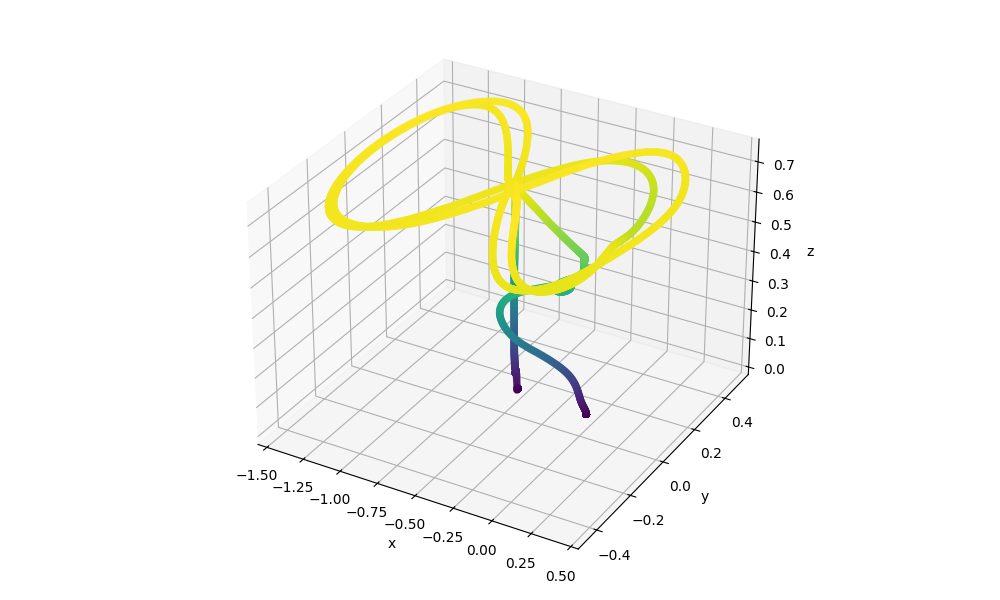
\includegraphics[width=\textwidth]{imgs/task2_mocap.png}
        \caption{Direct MoCap Position}
    \end{subfigure}
    \begin{subfigure}{0.45\textwidth}
        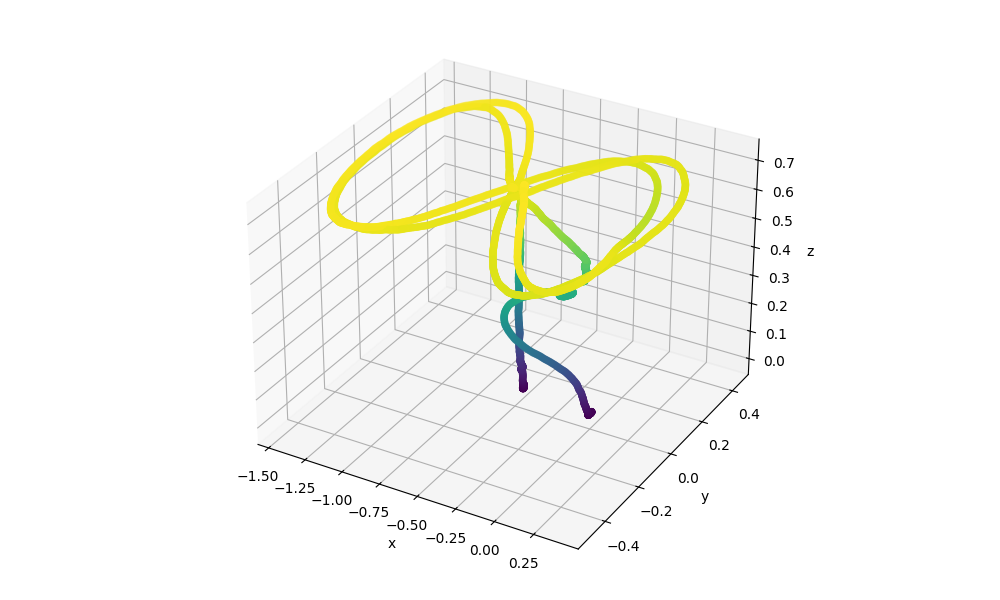
\includegraphics[width=\textwidth]{imgs/task2_velocity.png}
        \caption{Direct MoCap Velocity}
    \end{subfigure}
    \begin{subfigure}{0.45\textwidth}
        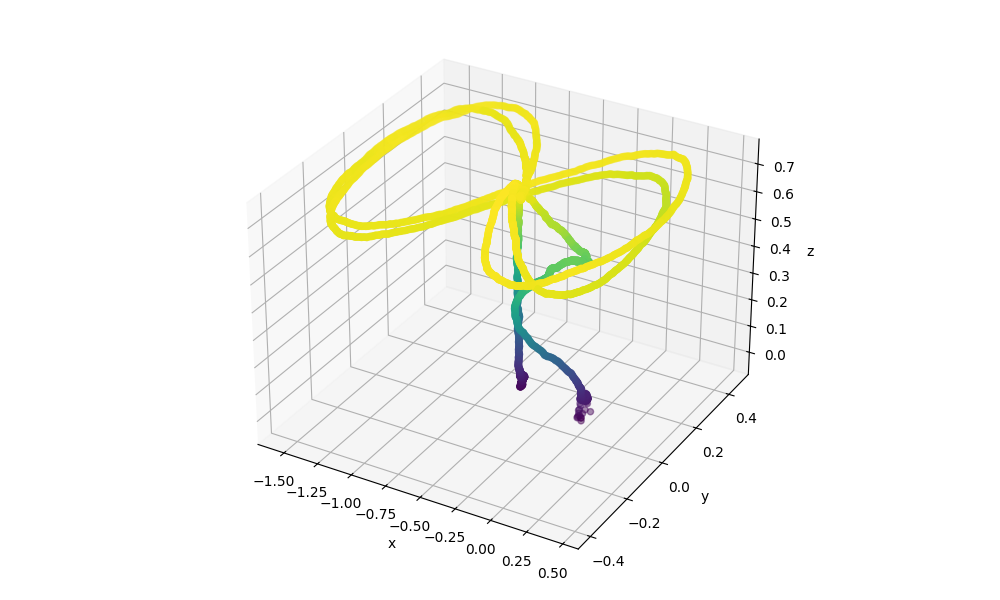
\includegraphics[width=\textwidth]{imgs/task2_low_noise.png}
        \caption{Low Noise}
    \end{subfigure}
    \begin{subfigure}{0.45\textwidth}
        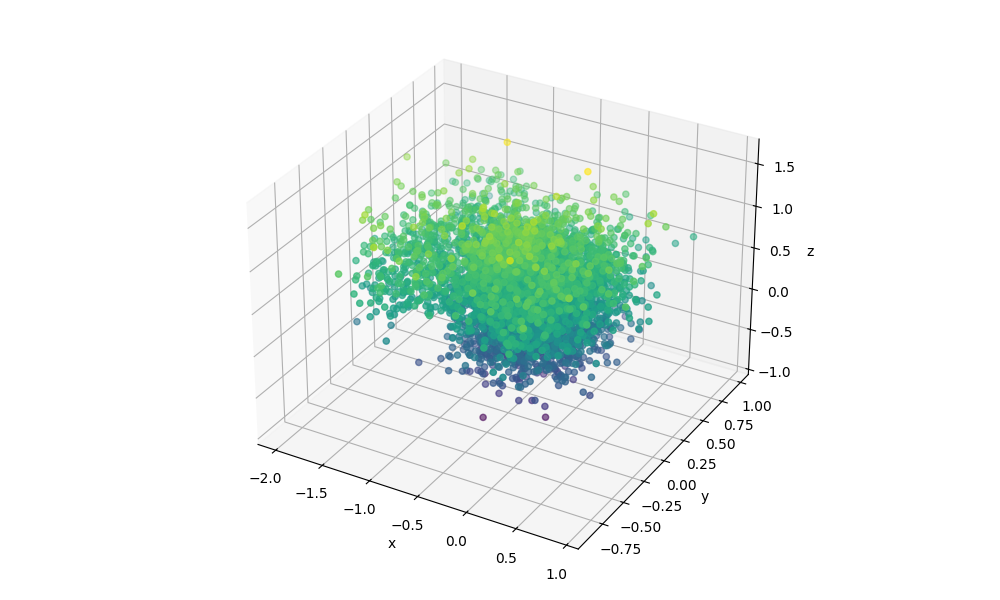
\includegraphics[width=\textwidth]{imgs/task2_high_noise.png}
        \caption{High Noise}
    \end{subfigure}
    \caption{Kalman Filter results}
\end{figure}

Here we see that as noise is added, the precise trajectory tracking becomes cloudier, with the Kalman filter attempting to simplify and smooth the trajectories.

\end{document}